% Draw horizonal line of nodes
\newcommand{\DrawHoriz}[2]{
    \draw[gray, thin] (-0.5, #1)
    -- ++(0.5, 0) node [pos=0.0, #2] {}
    -- ++(1.0, 0) node [pos=0.5, #2] {}
    -- ++(1.0, 0) node [pos=0.5, #2] {}
    -- ++(1.0, 0) node [pos=0.5, #2] {}
    -- ++(0.5, 0) node [pos=1.0, #2] {};
}
% Draw vertical line of nodes
\newcommand{\DrawVert}[2]{
    \draw[gray, thin] (#1, -0.5)
    -- ++(0, 0.5) node [pos=0.0, #2] {}
    -- ++(0, 1.0) node [pos=0.5, #2] {}
    -- ++(0, 1.0) node [pos=0.5, #2] {}
    -- ++(0, 1.0) node [pos=0.5, #2] {}
    -- ++(0, 0.5) node [pos=1.0, #2] {};
}
% Draw grid
\newcommand{\DrawGrid}[1]{
    \foreach \x in {0,...,3} \DrawHoriz{\x}{#1};
    \foreach \y in {0,...,3} \DrawVert{\y}{#1};
}

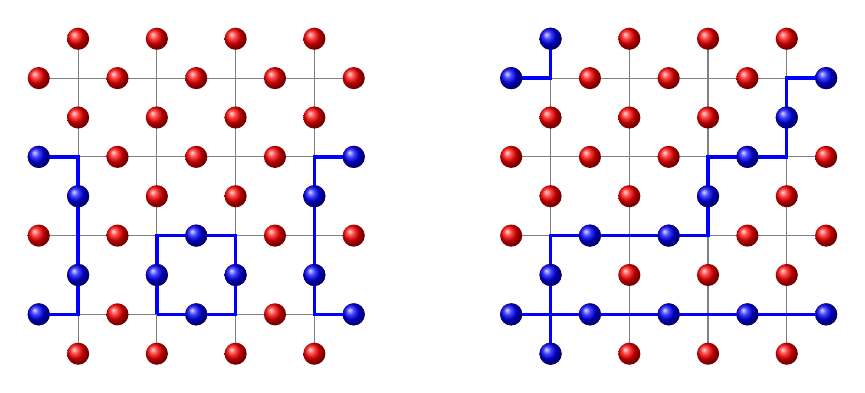
\begin{tikzpicture}[
        ball/.style={shade, shading=ball, circle, minimum size=8pt, inner sep=0pt},
        zero/.style={ball, ball color=red},
        one/.style={ball, ball color=blue},
        loopline/.style={blue, very thick},
        loopdot/.style={pos=0.5, one},
        loopstart/.style={pos=0, one},
        loopend/.style={pos=1, one}
    ]
  %%% First grid
  % Draw a grid of red dots
  \DrawGrid{zero};
  % Draw over loops of blue dots
  \draw[loopline]
  (1,0) foreach \x / \y in {1/0, 0/1, -1/0, 0/-1} { -- ++(\x, \y) node [loopdot] {} } ;
  \draw[loopline]
    (-0.5,0) -- (0,0) node [loopstart] {}
    foreach \y in {1, 1} { -- ++(0, \y) node [loopdot] {} }
    -- ++(-0.5, 0) node [loopend] {};
  \draw[loopline]
  (3.5,0) -- (3,0) node [loopstart] {}
  foreach \y in {1, 1} { -- ++(0, \y) node [loopdot] {} }
  -- ++(0.5, 0) node [loopend] {};

  %%% Second grid, shifted
  \begin{scope}[xshift=6cm]
      % Grid of red dots
      \DrawGrid{zero};
      % Loop
      \draw[loopline]
          (-0.5,0) -- (0,0) node [loopstart] {}
          foreach \x in {1, 2, 3} { -- (\x, 0) node [loopdot] {} }
          -- (3.5,0) node [loopend] {};
      \draw[loopline]
          (0,-0.5) -- (0,0) node [loopstart] {}
          foreach \x / \y in {0/1, 1/0, 1/0, 0/1, 1/0, 0/1} { -- ++(\x, \y) node [loopdot] {} }
          -- ++(0.5,0) node [loopend] {};
      \draw[loopline]
        (-0.5,3)  -- (0,3) node [loopstart] {}
        -- (0,3.5) node [loopend] {};
  \end{scope}
\end{tikzpicture}
